\subsection{Natural Joins}

The \emph{natural~join} \( R \bowtie S \) of two relations \( R \) and \( S \) is the set of all combinations of the tuples of \( R \) and \( S \) whose common attributes are equal.

\begin{figure}[htp]
  \centering
  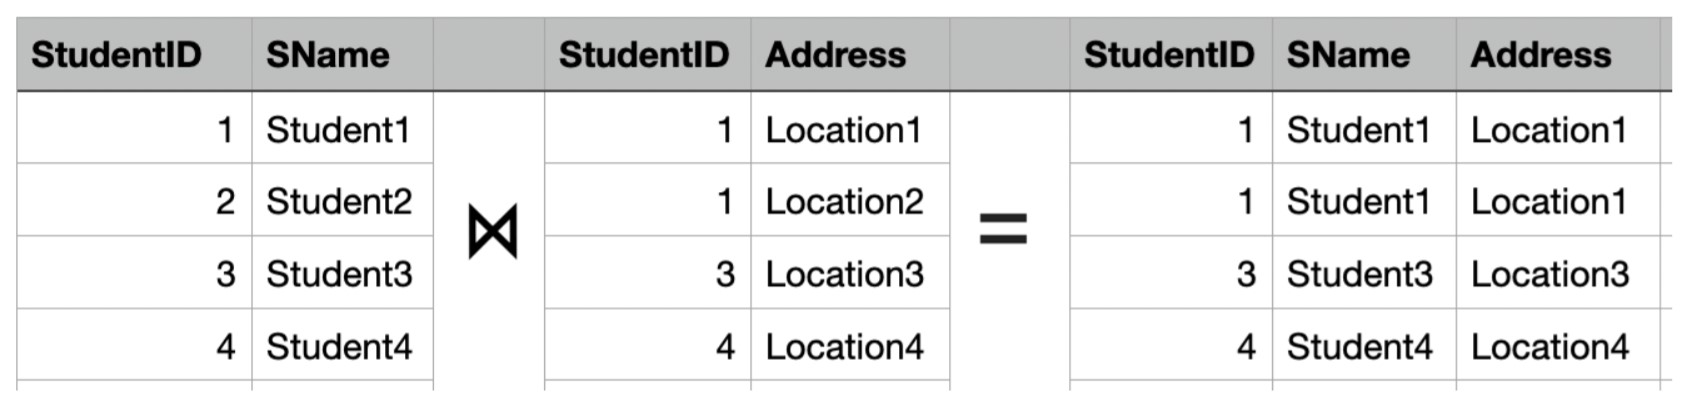
\includegraphics[width=0.8\textwidth]{unit-3/figures/natural-join.jpg}
  \caption*{The natural join of two relations.}
\end{figure}

\subsection{Decomposition of a Relation}

The decomposition of a relation \( R \), whose attributes are the set \( \itol{A} = \left\{ a_1, a_2, \ldots, a_m \right\} \), results in the creation of two new relations \( R_1 \) and \( R_2 \), whose attributes are the sets \( \itol{B} = \left\{ b_1, b_2, \ldots, b_n \right\} \) and \( \itol{C} = \left\{ c_1, c_2, \ldots, c_p \right\} \), respectively, such that \( R_1 \) and \( R_2 \) together contain all the attributes of \( R \), and the natural~join of \( R_1 \) and \( R_2 \) gives \( R \) exactly --- no more, no less.

Thus, all decomposed relations exhibit the following properties.
\begin{equation*}
  \itol{B} \cup \itol{C} = \itol{A}
\end{equation*}
\begin{equation*}
  R_1 \bowtie R_2 = R
\end{equation*}

\subsection{Identification of Boyce-Codd Normal Form (BCNF)}

A relation \( R \) is in \emph{Boyce-Codd Normal Form (BCNF)} if, and only if, for each of its functional dependencies \( \itol{A} \rightarrow \itol{B} \), \( \itol{A} \) is a key.

A functional dependency that causes a relation not to be in BCNF is called a \emph{BCNF~violation}.

\subsection{BCNF Decomposition Algorithm}

In order to decompose the relation \( R \),
\begin{enumerate}
  \item compute the keys of \( R \), then
  \item until all relations are in BCNF,
  \begin{enumerate}
    \item pick any of the problem relations \( R' \) with at least one functional dependency \( \itol{A} \rightarrow \itol{B} \) that violates BCNF (where \( \itol{A} \) is not a key),
    \item decompose it into two relations \( R_1\!\left( \itol{A}, \itol{B} \right) \) and \( R_2\!\left( \itol{A}, \text{rest} \right) \) --- discarding the original relation \( R' \), then
    \item compute the functional dependencies of \( R'_1 \) and \( R'_2 \), and
    \item compute the keys of \( R'_1 \) and \( R'_2 \).
  \end{enumerate}
  \item Finally, the remaining relations \( R' \) are the decomposition of the original relation \( R \).
\end{enumerate}

\begin{figure}[htp]
  \centering
  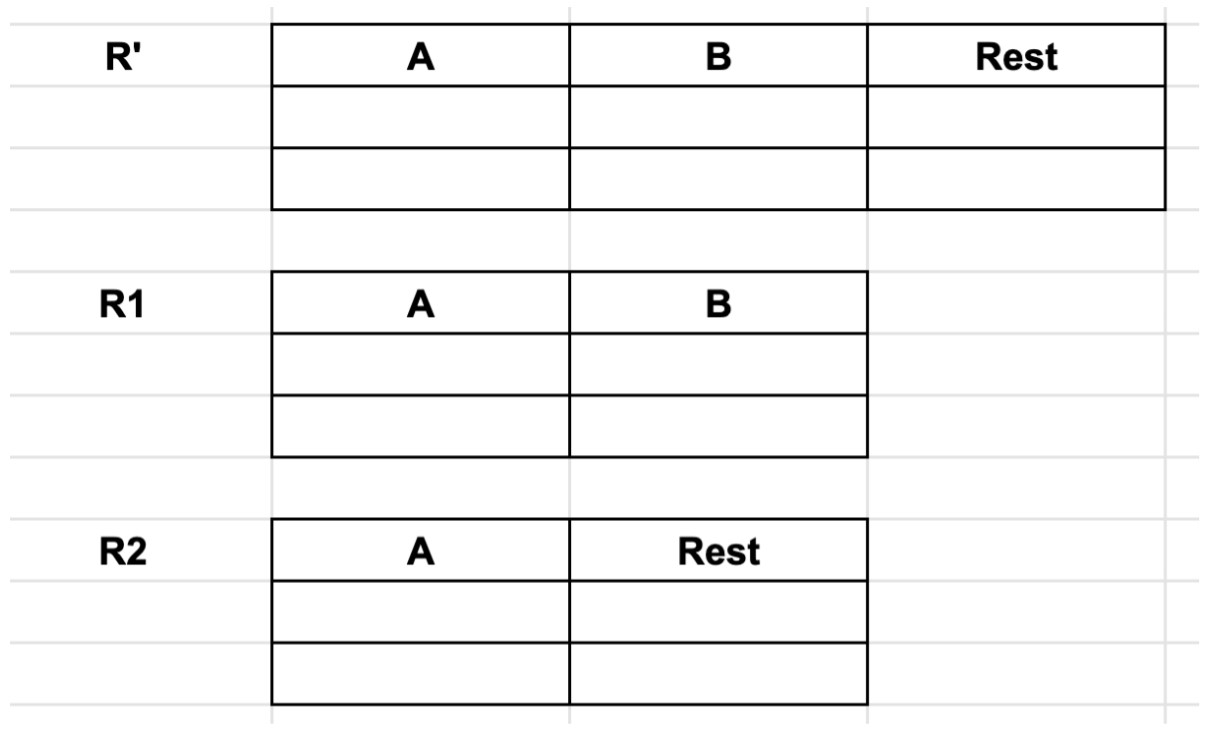
\includegraphics[width=0.6\textwidth]{unit-3/figures/decomposition.jpg}
  \caption*{Decomposition of a relation \( R'\!\left( \itol{A}, \itol{B}, \text{rest} \right) \) into \( R'_1\!\left( \itol{A}, \itol{B} \right) \) and \( R'_2\!\left( \itol{A}, \text{rest} \right) \).}
\end{figure}

The natural join of the decomposed relations \( R' \) is the original relation \( R \), and the union of the attributes of all \( R' \) is the set of attributes of \( R \).

BCNF provides the termination condition for decomposition.
A relation should be decomposed only if at least one of its functional dependencies is a BCNF~violation, and decomposition must continue until all relations are in BCNF, i.e. until there exists no relation with a functional dependency whose independent attributes are not a key.
